Cytoscape~可以读取以下格式的网络或路径文件:
\begin{itemize}
\item Simple interaction file (SIF or .sif format) 
\item Graph Markup Language (GML or .gml format) 
\item XGMML (extensible graph markup and modelling language). 
\item SBML 
\item BioPAX 
\item PSI-MI Level 1 and 2.5 
\item Delimited text 
\item Excel Workbook (.xls) 
\end{itemize}

SIF~格式的文件只有节点和相互作用,而其它的格式都可以存储网络布局信息,还可以跟其它的网络软件和数据源交换数据。SIF~文件通常用于在新建网络时导入相互作用,因为用文本编辑器和电子表格软件能很方便的创建这种格式的文件。在导入了相互作用,应用了某种网络布局后,就可以将网络存为GML或XGMML格式,从而能去其它系统交换数据。所有的这些格式(Excel例外)都是文本文件,用普通的文本编辑器就能编辑和查看这些文件。


\section{SIF~格式}
这种简单的格式可以很方便地用于从相互作用列表构建网络。利用这种格式,还能很方便的把小网络组合在一起,或是在现有的数据中添加新的相互作用。但这种格式的缺点也是显而易见的,其中不包含布局信息,这使得Cytoscape不得不在每次加载网络时都重新计算网络的布局。

SIF~文件中的每行都由起点、相互作用类型(或边的类型)和一个或若干个重点构成。
\begin{verbatim}
nodeA <relationship type> nodeB
nodeC <relationship type> nodeA
nodeD <relationship type> nodeE nodeF nodeB
nodeG
...
nodeY <relationship type> nodeZ
\end{verbatim}

下面是一个具体的例子:
 \begin{verbatim}
node1 typeA node2
node2 typeB node3 node4 node5
node0
\end{verbatim}

第一行是两个节点,node1和node2,以及两点间的typeA型的相互关系。第二行加入了三个新节点,node3~、\linebreak node4~和~node5,这一行中的node2跟第一行中的node2是同一个节点。第二行还设定了三条起点相同且类型也相同的相互作用。第三行说明了如何引入孤立的节点。 This form is not needed for nodes that do have relationships, since the specification of the relationship implicitly identifies the nodes as well. 

重复的条目被忽略。两个点之间的多条相互作用必须是不同的类型。例如,下面的node1和node2之间就有两条边,但类型分别是xx和yy。
\begin{verbatim}
node1 xx node2
node1 xx node2
node1 yy node2
\end{verbatim}

节点的自相互作用是允许的:
\begin{verbatim}
node1 xx node1
\end{verbatim}

Cytoscape中每个点和每条边都有标识符,通常在节点和边的属性数据中都有。节点的名称必须是独一无二的,名称相同的节点会被视为同一个节点。节点的名称缺省情况下就是文件中的名称,除非用Visual Mapper映射到了其他字符串。详见``视觉风格''一章。边的名称则是由边的起点和终点,加上相互作用的类型构成的,例如:sourceName (edgeType) targetName。


$<$relationship type$>$标签可以是任何字符串。完整的单词或是单词的组合都可以用来定义相互作用的类型,例如:geneFusion、cogInference、pullsDown、activates、degrades、inactivates~、~inhibits~、~phosphorylates~、~upRegulates~等等。 

在系统生物学领域,常见的相互作用类型有:
\begin{enumerate}
\item  pp .................. protein $\rightarrow$ protein interaction
\item  pd .................. protein $\rightarrow$ DNA   
  (例如,转录因子跟调控基因的上游结合。)
\end{enumerate}

还有一些相对少见的相互作用类型:
\begin{enumerate}
\item  pr .................. protein $\rightarrow$ reaction
\item  rc .................. reaction $\rightarrow$ compound
\item  cr .................. compound $\rightarrow$ reaction
\item  gl .................. genetic lethal relationship
\item  pm .................. protein-metabolite interaction
\item  mp .................. metabolite-protein interaction
\end{enumerate}


\textbf{分隔符}

在简单的相互作用文件格式中,空白(空格或制表符)用来分割名称。但在有些情况,节点名称或是边的类型中会含有空格。Cytoscape对分隔符的处理原则是这样的:如果文件中有制表符,那么就用制表符分割不同的字段,而空格则被视为字段中的内容。如果文件中没有制表符,那么所有的空格就都是分隔符(也就是中字段中不会有空格)。

如果在导入网路后,发现网络中没有边,而且点的名称也有问题,那很有可能是因为文件中存在制表符,使得Cytoscape在导入网络时判断错误。另一方面,如果网络中节点的名称只是正确名称的一部分,那就很有可能是错误地将空格作为了分隔符,实际上应该用制表符。

用简单的相互作用的形式存放网络的文件的后缀是.sif,Cytoscape能识别出文件夹中所含有的这类文件。

\section{GML~格式}
跟SIF格式不同,GML是一种富图格式语言(rich graph format language),很多网络可视化软件包都支持这种格式。在\url{http://www.infosun.fmi.uni-passau.de/Graphlet/GML/}上可以找到该格式的具体说明。

通常都不必直接修改GML文件的内容。当SIF格式的网络导入并实施布局后,就可以以GML的形式保存和加载网络。GML文件中的视觉风格在加载GML文件后,会保存为名为Filename.style的视觉风格。

\section{XGMML~格式}
XGMML是GML的XML扩展版,它是基于GML定义的。除了网络数据,XGMML还包含节点、边和网络的属性。XGMML文件的规范在\url{http://www.cs.rpi.edu/~puninj/XGMML/}上。

由于XGMML继承了XML文件的灵活性,所以XGMML比GML更受欢迎。如果不确定应该用哪种格式,那就选择XGMML吧。

\section{系统生物学标记语言(Systems Biology Markup Language)}
系统生物学标记语言(Systems Biology Markup language)是一种用于描述生化网络的XML格式。SBML文件格式规范:\url{http://sbml.org/documents/}
 
\section{BioPAX (Biological PAthways eXchange)格式}

BioPAX是一种用于交换生物路径数据的OWL(Web Ontology Language)文档。该格式的完整说明文档:\url{http://www.biopax.org/index.html}

\section{PSI-MI~格式}
PSI-MI格式一种用于描述蛋白质相互作用及有关数据的XML格式。PSI-MI XML的格式规范:
\url{http://psidev.sourceforge.net/mi/xml/doc/user/}。

\section{纯文本表格和Excel表格}

Cytoscape~为微软的Excel文件(.xls)和纯文本表格提供了原生支持。可以用这些表格存储网络数据和边的属性。在导入文件的过程中,用户可以指定哪一列是源节点,哪一列是终点,以及相互作用的类型、边属性等等。其它的一些网络分析工具,例如igraph (\url{http://cneurocvs.rmki.kfki.hu/igraph/}), 也可以将网络输出成简单的文本文件。Cytoscape~可以读取这些文本文件,并构建网络。具体信息请阅读\ref{free-format table} 节。

\centerline{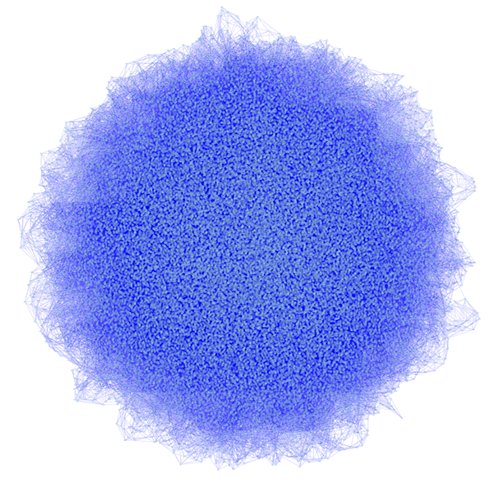
\includegraphics[width=.7\textwidth]{images/huge_network_igraph.png}}

\textbf{在Cytoscape中显示根据~igraph~的Watts-Strogatz小世界模型生成的网络(含有5万个节点,25万条边)}
 
利用Table Import功能,可以读取其它软件生成的网络。
 
\section{Cytoscape~中节点的命名}

通常情况下,节点表示基因,节点间的边表示相互作用(或者是其他的生物关系)。
为了紧凑,基因也可以表示成响应的蛋白质。节点还可以用来表示化合物和生化反应等各种
东西,并不局限于基因。

如果想要将网络中的基因或蛋白跟GO注释或基因表达数据整合在一起,那各个数据文件中的基因名称
必须完全一致。我们强烈建议用户用ORF系统名称或是标准的获取编号(accession number)来命名
基因和蛋白质。而常用名称(common name)由于更适合显示在屏幕上,所以可以将其存放在注释目录或
节点的属性文件中。Cytoscape的annotation/目录中中有酵母的ORF到常用名称的对应文件。将来会逐步
地支持其它物种。

为什么要建议使用标准的基因名称?所有~Cytoscape~能识别的外部数据格式都有专门的命名方式。例如,
蛋白质相互作用网络会列出蛋白质的名称,相应的属性和表达数据也使用同样的命名方法。

但如果要把不用来源的数据结合在一起,问题就出现了:对于同一个东西,不同的数据源的命名可能
是不一样的。例如,基因就可以有多个不同的名称,包括正式的``染色体位置''标识符,研究人员讨论
时常用的若干个名称。此外,每个数据库可能还会有自己的一套给基因编号的方法(例如Swiss-Prot的
蛋白质编号)。如果一个数据源使用的是正式名称,而另一个数据使用的是常用名称,那Cytoscape就必须
要知道哪两个名称指的是同一个基因。

有两种方法来解决这个问题,一个较简单,另一个稍微复杂一些。简单的方法就是假设所有的数据源使用同样
的命名方法。如果是这样,Cytoscape就能很方便的将来自不同数据源的数据结合在一起。

跟人工整合不同来源的数据一样,为了处理不同命名方式的数据,Cytoscape需要同义词信息(见``注释
''一章)。同义词表提供了某个物种的每个对象的权威名称,以及相应的其它可以识别的名称。要注意,同义词表
自身的数据就是按照这个``权威''名称命名的。例如,在酵母中,通常用ORF名称作为这个``权威''名称。

如果能提供这样信息,Cytoscape在缺省情况下会将所有的名称都转换成相应的权威名称。而不能识别的名称
则保持不变。这样Cytoscape就能将不同来源的数据结合在一起,即使它们的名称不同也没关系---只要能在同义词
表中找到就行。

除了上面的数据,还需告诉Cytoscape各个对象所属的物种,因为数据服务器需要物种信息才能找到
相应的名称。通过Cytoscape的命令行选项-P(cytoscape.sh -P ``defaultSpeciesName=Saccharomyces
cerevisiae''), 或是编辑网络的属性(Edit $\rightarrow$ Preferences
$\rightarrow$ Properties\ldots)都可以设定网络的物种。 

通过-P选项(cytoscape.sh -P ``canonicalizeName=false'')或是编辑属性(Edit
$\rightarrow$ Preferences $\rightarrow$
Properties\ldots)以关闭名称的自动映射。
在当前的版本中,名称映射对基因表达数据无效。基因表达数据应该使用跟其它数据源相同的命名方式,伙食使用同义词表中的权威名称。
